\documentclass[11pt]{article}
\usepackage{latexsym}
\usepackage{amsmath}
\usepackage{amssymb}
\usepackage{amsthm}
\usepackage{epsfig}
\usepackage[tight]{subfigure}

\usepackage{amsmath}

\DeclareMathOperator*{\minimize}{min}
\DeclareMathOperator*{\maximize}{max}

\DeclareMathOperator*{\argmax}{argmax} % thin space, limits underneath in displays
\DeclareMathOperator*{\argmin}{argmin}

\usepackage{algorithm}
 %on linux you may need to run sudo apt-get install texlive-full to install algorithm.sys
\usepackage{algorithmic}

\usepackage{verbatim}
\usepackage{amsmath,amsfonts,amsthm,bm}


\newcommand{\handout}[5]{
  \noindent
  \begin{center}
  \framebox{
    \vbox{
      \hbox to 5.78in { {#1} \hfill #2 }
      \vspace{4mm}
      \hbox to 5.78in { {\Large \hfill #5  \hfill} }
      \vspace{2mm}
      \hbox to 5.78in { {\em #3 \hfill #4} }
    }
  }
  \end{center}
  \vspace*{4mm}
}

\newcommand{\lecture}[5]{\handout{#1}{#2}{#3}{#4}{#5}}
\newcommand{\collision}[0]{\mathrm{collision}}
\newcommand{\nocollision}[0]{\overline{\collision}}

\newcommand*{\QED}{\hfill\ensuremath{\square}}

\newtheorem{theorem}{Theorem}
\newtheorem{corollary}[theorem]{Corollary}
\newtheorem{lemma}[theorem]{Lemma}
\newtheorem{observation}[theorem]{Observation}
\newtheorem{proposition}[theorem]{Proposition}
\newtheorem{definition}[theorem]{Definition}
\newtheorem{claim}[theorem]{Claim}
\newtheorem{fact}[theorem]{Fact}
\newtheorem{assumption}[theorem]{Assumption}
\newtheorem{note}[theorem]{Note}

% 1-inch margins, from fullpage.sty by H.Partl, Version 2, Dec. 15, 1988.
\topmargin 0pt
\advance \topmargin by -\headheight
\advance \topmargin by -\headsep
\textheight 8.9in
\oddsidemargin 0pt
\evensidemargin \oddsidemargin
\marginparwidth 0.5in
\textwidth 6.5in

\parindent 0in
\parskip 1.5ex
%\renewcommand{\baselinestretch}{1.25}

\newcommand{\btheta}{\boldsymbol{\theta}}
\newcommand{\bz}{\boldsymbol{z}}
\newcommand{\bw}{\boldsymbol{w}}
\newcommand{\bu}{\boldsymbol{u}}
\newcommand{\bv}{\boldsymbol{v}}
\newcommand{\bx}{\boldsymbol{x}}


% \newcommand{\argmin}[1]{\underset{#1}{\operatorname{arg}\,\operatorname{min}}\;}
% \newcommand{\argmax}[1]{\underset{#1}{\operatorname{arg}\,\operatorname{max}}\;}

\begin{document}

\lecture{Statistical Techniques in Robotics (16-831, S22)}{Lecture \#21
  (Wednesday, April 6)}{Lecturer: Kris Kitani}{Scribes: Jia Shi, Mukun Guo}{Policy Gradient Method and Actor-Critic}

\section{Review}
%This section serves as a review of the previous lecture and any other context required to frame the content of the current lecture. 

%You may format the scribes in any way you like, aside from changing font style, size and page format. Please use subsections and paragraphs to increase the readability of your notes.

%Length requirement 1-2 pages.

In Last lecture, we talked about model-free value-based control and moved from discrete space to continuous space. On a high level, in discrete cases, we can store the Q-values for each state-action pair, whereas in continuous space such pairs are infinite. Thus, we use a function approximator to map each state-action pair to a value. In this section, we briefly review some important concepts from last lecture.

\subsection{Function Approximator for Control}
In previous lectures, we have discussed many model-free value-based control algorithms (i.e. Monte Carlo Control, TD Control, On-policy/Off-policy, etc), but we limited our discussion in a discrete setup, where we can essentially store the value function for every state-action pair in a table. However, there are always cases where the state/action space is continuous. In such setup, we will replace the table with a function approximator. There are many choices for such function approximator. The current most popular one in research communities are deep neural networks. Specifically, previously we store the $Q^\pi(s, a)$ value for every state-action pair. In every time step, we update the value itself using some algorithm. Now we will approximate $Q^\pi(s,a)$ using a function $Q_\theta (s, a)$ that is paramterized by $\theta$, and in ever time step we will update $\theta$ so that the function better approximate the value function $Q^\pi(s,a)$.

\subsubsection{Control algorithms in Continuous space}
Monte Carlo Control algorithm in continuous space is very similar to the discrete space, with two modifications.
\begin{enumerate}
    \item Instead of updating the Q-value for each state-action pair: $$Q\left(a^{(t)}, s^{(t)}\right) \leftarrow Q\left(a^{(t)}, s^{(t)}\right)+\alpha\left[G^{(t)}-Q\left(a^{(t)}, s^{(t)}\right)\right]$$ we will instead update the parameters of the approximator function: $$\theta=\theta+\alpha\left(G^{(t)}-Q_{\theta}\left(s^{(t)}, a^{(t)}\right)\right) \frac{\partial}{\partial \theta} Q_{\theta}\left(s^{(t)}, a^{(t)}\right)$$ Note that in MC Control, $G^{(t)}$ is simply the cumulative return. Its value is independent of the space being continuous or discrete.
    \item We also need to add stochasticity into the policy. Specifically, at the beginning of each episode, with probability $\epsilon$, a random policy will be applied where actions will be randomly selected. With probability $(1-\epsilon)$, we apply a greedy policy where we always select the action with highest value given by our approximator function $Q_\theta(s, a)$, that is, $a^* = \argmax_a Q_\theta(s, a)$.
\end{enumerate}
For On-policy TD Control (SARSA), similar modifications were made with some slight change.
\begin{enumerate}
    \item We apply same parameter update as MC Control
    \item Instead select policy at the beginning of each episode, the sampling is done at the beginning of every epoch. The sample strategy is the same as MC Control.
    \item Since in TD Control, we use an estimator which uses $Q(s, a)$ to estimate $G^{(t)}$, we need to slightly modify how the estimator works. But this is very simple and straightforward. Originally, our one-step TD uses $$G^{(t)} \leftarrow r^{(t)}+\gamma Q\left(a^{(t+1)}, s^{(t+1)}\right)$$ to estimate the return. We simply replace the Q-value with the approximator function: $$G^{(t)} \leftarrow r^{(t)}+\gamma Q_{\theta}\left(a^{(t+1)}, s^{(t+1)}\right)$$
\end{enumerate}
The Off-policy TD Control in continuous space is same as the On-policy version, except for the policy sampling is done on the behavior policy $\mu$.

\subsubsection{Framework for Function Approximation for Control}
With the above concrete examples, we notice that the modification from discrete to continuous space can be generalize into 3 steps:
\begin{enumerate}
    \item Apply an approximator function $Q_{\theta}(s, a) \approx Q^{\pi}(s, a)$.
    \item Set up optimization problem with objective function: $\hat{\boldsymbol{\theta}}=\underset{\theta}{\arg \min } \mathbb{E}_{p}\left[\left(Q^{\pi}(s, a)-Q_{\theta}(s, a)\right)^{2}\right]$, find the solution using SGD $$\nabla_{\theta} \mathcal{L}_{\theta} \approx-\left(Q^{\pi}(s, a)-Q_{\theta}(s, a)\right) \frac{\partial}{\partial \theta} Q_{\theta}(s, a)$$ $$\theta=\theta-\alpha\nabla_{\theta} \mathcal{L}_{\theta}$$
    \item Select a return estimator (Monte Carlo, TD, etc) to estimate $Q^{\pi}(s, a)$ to run the SGD: $$Q^{\pi}(s, a) \approx G^{(t)}$$
\end{enumerate}


\section{Summary}
\subsection{Policy Gradient Method}
We have concluded out study on Value-based Reinforcement Learning. We will not move into a new domain, Policy-based RL. In policy gradient methods, we skip estimation of the value function and directly learns a function $\pi_\theta(a|s)$ that approximates the best policy. Recall that our ultimate objective is to maximize the return by playing with the parameters of the policy function. Formally, we could set up the following optimization problem: $$\hat{\theta}=\underset{\theta}{\arg \max } \mathbb{E}_{p_{\theta}(\zeta)}\left[\sum_{t=0}^{T} r^{(t)}\right]$$ where $p_{\theta}(\zeta)$ is the distribution over trajectories under MDP: 
\begin{align*}
    p_{\theta}(\zeta)&=p\left(s^{(0)}\right) \Pi_{t=0}^{T} \pi_{\theta}\left(a^{(t)} \mid s^{(t)}\right) p\left(s^{(t+1)} \mid s^{(t)}, a^{(t)}\right) \\
\zeta&=\left\{s^{(0)}, a^{(0)}, s^{(1)}, a^{(1)}, \ldots, s^{(T)}, a^{(T)}\right\} \\
r^{(t)} &\triangleq r\left(s^{(t+1)}, a^{(t)}, s^{(t)}\right)
\end{align*}
Note that this is a maximization problem. Hence we will apply gradient ascent to solve it. Let's set $$J(\theta) = \mathbb{E}_{p_{\theta}(\zeta)}\left[\sum_{t=0}^{T} r^{(t)}\right]$$
Apply first-order Taylor Series approximation with quadratic regularization $$\hat{\theta}=\underset{\theta}{\arg \max }\left\{\alpha\left(J\left(\theta^{\prime}\right)+\left\langle\theta-\theta^{\prime}, \nabla_{\theta^{\prime}} J\left(\theta^{\prime}\right)\right)-\frac{1}{2}\left\|\theta-\theta^{\prime}\right\|^{2}\right\}\right.$$ 
Now let's try to solve this new optimization problem using closed-form:
\begin{align*}
\nabla_{\theta}\left\{\alpha\left(J\left(\theta^{\prime}\right)+\left\langle\theta-\theta^{\prime}, \nabla_{\theta^{\prime}} J\left(\theta^{\prime}\right)\right\rangle\right)-\frac{1}{2}\left\|\theta-\theta^{\prime}\right\|^{2}\right\}&=0 \\
\alpha \nabla_{\theta^{\prime}} J\left(\theta^{\prime}\right)-\theta+\theta^{\prime} &=0
\end{align*}
Rearrange the terms we could get the following gradient update rule:
$$\theta \leftarrow \theta^{\prime}+\alpha \nabla_{\theta^{\prime}} J\left(\theta^{\prime}\right)$$
Now Let's take a look at that's inside the gradient term $\nabla_{\theta^{\prime}} J\left(\theta^{\prime}\right)$. Recall that
$$J(\theta)=\mathbb{E}_{p_{\theta}(\zeta)}\left[\sum_{t=0}^{T} r^{(t)}\right]=\int_{\zeta} p_{\theta}(\zeta) r(\zeta) d \zeta$$ where $r(\zeta)=\sum_{t=0}^{T} r^{(t)}$. Take its derivative w.r.t. $\theta$ and apply some basic derivative rules:
\begin{align*}
\nabla_{\theta} J(\theta) &=\nabla_{\theta} \int_{\theta} p_{\theta}(\zeta) r(\zeta) d \zeta  \\
&=\int_{\theta} \nabla_{\theta} p_{\theta}(\zeta) r(\zeta) d \zeta \\
&=\int_{\theta} p_{\theta}(\zeta) \frac{\nabla_{\theta} p_{\theta}(\zeta)}{p_{\theta}(\zeta)} r(\zeta) d \zeta \\
&=\int_{\theta} p_{\theta}(\zeta) \nabla_{\theta} \ln p_{\theta}(\zeta) r(\zeta) d \zeta
\end{align*}
Recall that a trajectory is simply a combination of state-actions pairs modeled by the MDP, that is, 
$$p(\zeta) = p(s^{(0)}) \prod_t \left[\pi_\theta(a^{(t)} | s^{(t)}) \cdot p(s^{(t+1)} | s^{(t)}, a^{(t)})\right]$$
Since we are in the log space, this becomes:
$$\ln p(\zeta) = \ln p(s^{(0)}) + \sum_t \left[\ln \pi_\theta(a^{(t)} | s^{(t)}) + \ln p(s^{(t+1)} | s^{(t)}, a^{(t)})\right]$$
Thus, we have:
$$\nabla_{\theta} \ln p_{\theta}(\zeta) =\nabla_{\theta}\left[\ln p\left(s^{(0)}\right)+\sum_{t=1}^{T} \ln \pi_{\theta}\left(a^{(t)} \mid s^{(t)}\right)+\ln p\left(s^{(t+1)} \mid s^{(t)}, a^{(t)}\right)\right] $$ 
Note that only the second term (i.e. policy) depend on $\theta$,
$$\nabla_{\theta} \ln p_{\theta}(\zeta) =\nabla_{\theta}\left[\sum_{t=1}^{T} \ln \pi_{\theta}\left(a^{(t)} \mid s^{(t)}\right)\right]$$
Plug it into the gradient term, we have:
\begin{align*}
\nabla_{\theta} J(\theta) &=\int_{\theta} p_{\theta}(\zeta) \nabla_{\theta}\left[\sum_{t=1}^{T} \ln \pi_{\theta}\left(a^{(t)} \mid s^{(t)}\right)\right] r(\zeta) d \zeta \\
 &=\mathbb{E}_{p_{\theta}}\left[\left(\sum_{t=1}^{T} \nabla_{\theta} \ln \pi_{\theta}\left(a^{(t)} \mid s^{(t)}\right)\right) r(\zeta)\right]
\end{align*} 
Note that above is an theoretical expectation term and in reality is very hard to obtain. Hence we replace the expectation with a simple average over trajectories (i.e. \textbf{Monte-Carlo Estimation}):
$$\nabla_{\theta} J(\theta) \approx \frac{1}{N} \sum_{n=1}^{N} \left[\left(\sum_{t=1}^{T} \nabla_{\theta} \ln \pi_{\theta}\left(a^{(t)} \mid s^{(t)}\right)\right) r(\zeta)\right]$$
Now let's try to understand this gradient term part by part. $r(\zeta) = \left(\sum_{t=1}^{T} r^{(t)}\right)$ is nothing more than the cumulative return of an episode (i.e. \textbf{Episodic Return}). The higher the return, the larger the gradient term. This essentially indicates how good the current policy is. If it's a good policy, we will have high return and update the policy function with larger gradient value in this direction. If the policy is bad, $r(\zeta)$ will be small and we make little update. Furthermore, We claim that $\sum_{t=1}^{T} \nabla_{\theta} \ln \pi_{\theta}\left(a^{(t)} \mid s^{(t)}\right)$, the \textbf{Eligibility Vector}, is an unbiased estimator of the policy function, because $\nabla_{\theta} \ln \pi_{\theta}\left(a^{(t)} \mid s^{(t)}\right) = \frac{\nabla_{\theta} \pi_{\theta}\left(a^{(t)} \mid s^{(t)}\right)}{ \pi_{\theta}\left(a^{(t)} \mid s^{(t)}\right)}$ where the denominator is an inverse weighting. If some actions have lower probability, we will apply a larger weights as an offset and vice versa. This ensures for both lower-probability action and higher-probability action we have appropriate gradient values.

\subsection{Monte-Carlo Policy Gradient}
Now that we have finished all the pieces of gradient ascent, we can put together our first policy-based reinforcement learning algorithm.
\begin{algorithm}
\caption{function MC-POLICY-GRADIENT $\left(\pi_{\theta}, \alpha\right)$}\label{alg:alg1}
\begin{algorithmic}
\FOR{$e=1, \ldots, E$} 
\STATE $\left\{s^{(t)}, a^{(t)}, r^{(t)}\right\}_{t=0}^{T} \sim \mathcal{E} \mid \pi_{\theta}$
\STATE $G^{(0)}=\sum_{t=0}^{T} r^{(t)}$
\FOR{$t=0, \ldots, T$}
\STATE $\theta \leftarrow \theta+\alpha\left(\nabla_{\theta} \log \pi_{\theta}\left(a^{(t)} | s^{(t)}\right)\right)\left(G^{(0)}\right)$
\ENDFOR
\ENDFOR
\STATE return $\pi_{\theta}$
\end{algorithmic}
\end{algorithm}

\subsection{Episodic Reinforcement Algorithm}
Just like other Monte-Carlo algorithms, this policy gradient algorithm also suffers from high variance. Two tricks were proposed to tackle this issue.
\subsubsection{Enforce Causality}
Since the high variance comes from how return is estimated. We slightly modify the estimation such that the policy's decision at time $t$ cannot affect past rewards. Formally, 
\begin{align*}
    G^{(0)} &= \sum_{t=0}^{T} r^{(n, t)} \\
    &\downarrow \\
    G^{(0)} &= \sum_{t=t'}^{T} r^{(n, t)} 
\end{align*}
Before, whenever we want to update the policy, we considers how this update affects past, now, and future. With this slight tweak, out policy update now only takes into consideration of how current and future rewards change.

\subsection{Remove Gradient Bias with a baseline offset}
We now that high variance is partly cased by the large numerical value of the return. There is an even easier way to remove the high variance. We could simply subtract the return by some offset $b$ that does not depend on $\theta$. Formally, 
$$\nabla_{\theta} J(\theta)=\int_{\theta} p_{\theta}(\zeta) \nabla_{\theta} \ln p_{\theta}(\zeta)[r(\zeta)-b] d \zeta=\int_{\theta} p_{\theta}(\zeta) \nabla_{\theta} \ln p_{\theta}(\zeta) r(\zeta) d \zeta$$
The proof that subtracting $b$ does not affect gradient will be elaborated in Appendix. With this trick, we are ready to state the classic reinforcement algorithm! 
\begin{algorithm}
\caption{function Episodic-Reinforce $\left(\pi_{\theta}, \alpha\right)$}\label{alg:cap}
\begin{algorithmic}
\FOR{$e=1, \ldots, E$} 
\STATE $\left\{s^{(t)}, a^{(t)}, r^{(t)}\right\}_{t=0}^{T} \sim \mathcal{E} \mid \pi_{\theta}$
\STATE $G^{(0)}=\sum_{t=0}^{T} r^{(t)}$
\FOR{$t=0, \ldots, T$}
\STATE $\theta \leftarrow \theta+\alpha\left(\nabla_{\theta} \log \pi_{\theta}\left(a^{(t)} | s^{(t)}\right)\right)\left(G^{(0)} - b\right)$
\ENDFOR
\ENDFOR
\STATE return $\pi_{\theta}$
\end{algorithmic}
\end{algorithm}

If we put the two tricks together, we get the following policy gradient algorithm
\begin{algorithm}
\caption{function POLICY-GRADIENT $\left(\pi_{\theta}, \alpha\right)$}\label{alg:cap}
\begin{algorithmic}
\FOR{$e=1, \ldots, E$} 
\STATE $\left\{s^{(t)}, a^{(t)}, r^{(t)}\right\}_{t=0}^{T} \sim \mathcal{E} \mid \pi_{\theta}$
\FOR{$t=0, \ldots, T$}
\STATE $G^{(0)}=\sum_{i=t}^{T} r^{(i)}$
\STATE $\theta \leftarrow \theta+\alpha\left(\nabla_{\theta} \log \pi_{\theta}\left(a^{(t)} | s^{(t)}\right)\right)\left(G^{(0)}\right)$
\ENDFOR
\ENDFOR
\STATE return $\pi_{\theta}$
\end{algorithmic}
\end{algorithm}
With smaller variance, the gradient ascent converges faster and we can achieve good results with fewer sampled trajectories and episodes.

\subsection{Pros and Cons of Policy Gradient Methods}
\textbf{Pros:}
\begin{enumerate}
    \item Doesn't require model, learn from pure interaction with environment.
    \item Effective in high-dimensional or continuous action space.
    \item With specifically designed policy function, we can encode prior knowledge.
    \item Find the optimal stochastic policy and naturally explores due to inherent stochasticity. 
\end{enumerate}
\textbf{Cons:}
\begin{enumerate}
    \item Even with proposed tricks, gradient is still high variance and convergence is slow.
    \item Due to the nature of gradient ascent, smaller step size will lead to slow convergence. And we will probably converge in local maximum instead of global maximum. If we use a deep neural network at the policy function, we will also suffer from vanishing and exploding gradient.
\end{enumerate}
\subsection{Actor-Critic}
Actor-Critic is the hybrid of both policy base and value base method by calculating the optimal policy and value function at the same time. In the naming 'Actor-Critic', actor refers to the policy and critic refers to the reward function. It's the most popular RL algorithm.

In the policy gradient method, we need to run through the entire episode to calculate the return, as noted in term $\sum_{t=1}^{T}r^{(t)}$. Actor critic method provide a way to spare this effect by replacing the return with return estimator. Formally, 

\begin{align*}
    \nabla_\theta  J(\theta)&=\mathbb{E}_{p_\theta} \left[\left(\sum_{t=1}^{T}\nabla_{\theta}\ln_{\pi_ \theta}(a^{(t)}|s^{(t)})\right)\left( \sum_{t=1}^{T}r^{(t)}\right)\right] \\
    &\downarrow \\
    \nabla_\theta  J(\theta)&=\mathbb{E}_{p_\theta} \left[\left(\sum_{t=1}^{T}\nabla_{\theta}\ln_{\pi_ \theta}(a^{(t)}|s^{(t)})\right)\left( G_{\phi}^{(t)}\right)\right] 
\end{align*}

The $G_{\phi}^{(t)}$ is the function approximator, we can replace it with other method we have learn as list in Tab.\ref{Tab:func} to form other actor critic function. For instance, Algorithm \ref{algo:Q-MC-AC} shows where a Monte Carlo is applied as the function estimate, and Algorithm \ref{algo:Q-TD-AC} shows the case where a TD-function is applied, which line 5 is replaced with a one step return approximation of the Q function.


\begin{algorithm}[H]
\caption{Q-MC-ACTOR-CRITIC$( \pi_\theta , Q_\phi , \alpha , \beta)$}
\label{algo:Q-MC-AC}
\begin{algorithmic}[1]
\FOR{ $e= 1,...,E$}
\STATE $\{s^{(t)},a^{(t)},r^{(t)}\}_{t=0}^{T} \sim \mathcal{E}| \pi_\theta $
\FOR{ $t=0,..., T$}
\STATE $G^{(t)} \leftarrow \sum_{i=t}^{T} r^{(i)}$
\STATE $\phi \leftarrow \phi  +  \beta[ G^{(t)}-Q_\phi(a^{(t)} , s^ {( t )})]\nabla Q_\phi(a^{(t)} , s^{(t)})$
\STATE $\theta \leftarrow \theta + \alpha \nabla \log{\pi_\theta(a^{(t)}|s^{(t)})} \cdot Q_\phi(a^{(t)},s^{(t)}) $
\ENDFOR
\ENDFOR 
\RETURN $\pi_\theta$
\end{algorithmic}
\end{algorithm}


\begin{algorithm}[H]
\caption{Q-TD-ACTOR-CRITIC$( \pi_\theta , Q_\phi, \alpha, \beta)$}
\label{algo:Q-TD-AC}
\begin{algorithmic}[1]
\FOR{$ e=1,...,E$}
\STATE $ \{s^{(t)},a^{(t)},r^{(t)}\}_{t=0}^T  \sim \mathcal{E}| \pi_\theta $
\FOR{ $t=0,...,T$}
\STATE $ \delta  \leftarrow  r^{(t)} + Q_\phi( a^{(t+1)}, s^{(t+1)}) $
\STATE $ \phi  \leftarrow \phi + \beta[\delta-Q_\phi(a^{(t)},s^{(t)})]\nabla  Q_\phi(a^{(t)} , s^{(t)}) $
\STATE $ \theta \leftarrow \theta + \alpha \nabla_{ \theta } \log{\pi_\theta(a^{(t)}|s^{(t)})}  \cdot  Q_\phi(a^{(t)} , s^{(t)}) $
\ENDFOR
\ENDFOR 
\RETURN $ \pi_\theta$
\end{algorithmic}
\end{algorithm}

For the baseline offset term B in the gradient function $\nabla_\theta J(\theta)$, the optimal B offset we should use is the value function $V_{\phi}(s^{(t)})$ for which we can derive the optimal adjusted return, also known as the Advantage function $A(a^{(t)},s^{(t)})$, which is the difference between the policy gradient Q and the value function, formally, 
$$A(a^{(t)},s^{(t)})=Q_{\phi}(a^{(t)},s^{(t)})-V_{\phi}(s^{(t)})$$

Thus we have the full form of policy gradient with advantage function 
$$\nabla_\theta  J(\theta)=\mathbb{E}_{p_\theta} \left[\left(\sum_{t=1}^{T}\nabla_{\theta}\ln_{\pi_ \theta}(a^{(t)}|s^{(t)})\right)\left( \sum_{i=t}^{T}A_{\phi}(a,s)\right)\right] $$

\begin{table}[]
\centering
\begin{tabular}{|l|l|}
\hline
Method & Return estimator $G^{t}$ \\ \hline
MC     & $G^{(t)}=\sum_{i=t}^{T}r^{(i)}$                 \\ \hline
TD(0)     & $G^{(t)}_{0}= r^{t}+ \gamma V(s^{(t+1)})$                 \\ \hline
N-step TD & $G^{(t)}(N)=\sum_{i=t}^{t+N-1} \gamma^{i-t}r^{(i)} + \gamma^N V(s^{(t+N)})$\\ \hline
$\lambda-Return$ & $G^{(t)}_{\lambda}=(1-\lambda) \sum_{n=1}^{\infty} \lambda^{n-1}G^{(t)}(n)$                 \\ \hline
$TD(\lambda)$ & $G^{(t)}_{z} =z^{(t)}(s)\left[r^{(t)}+\gamma V(s^{(t+1)})\right]$                 \\ \hline
IS-MC      & $G^{(t)}_{\pi/\mu} =\prod_{i=t}^{T} \frac{\pi(a^{(i)}|s^{(i)})}{\mu(a^{(i)}|s^{(i)})} \sum_{j=t}^{T}r^{(j)}$                 \\ \hline
IS-TD(0) & $G^{(t)}_{\pi/\mu}(1)=\frac{\pi(a^{(i)}|s^{(i)})}{\mu(a^{(i)}|s^{(i)})} \left[r^{(t)}+\gamma V(s^{(t+1)})\right]$                 \\ \hline
\end{tabular}
\label{Tab:func}
\caption{Prediction methods to estimate return covered in class}
\end{table}

Algorithm \ref{algo:Advantage-MC-AC} give an example of advantage actor critic function with Monte Carlo estimator. In line the MC  estimator is obtained, and the parameter of value function, Q value function and the policy is updated with gradient decent algorithm in line 6,7,8 respectively.


\begin{algorithm}[H]
\caption{ADVANTAGE-MC-ACTOR-CRITIC$( \pi_\theta, Q_\phi, V_\psi, \alpha, \beta, \kappa)$}
\label{algo:Advantage-MC-AC}
\begin{algorithmic}[1]
\FOR{$ e = 1 ,...,E $}
\STATE $\{ s^{ (t)} , a^{(t)}, r^{(t)}\}_{t=0}^T \sim \mathcal{E}|\pi $
\FOR{$t = 0,...,T$}
\STATE $G^{(t)} \leftarrow  \sum_{i=t}^T  r^{(i)}$
\STATE $\psi  \leftarrow \psi  + \kappa[G^{(t)}-V_\phi(s^{(t)})]\nabla_\psi V_\psi(s^{(t)})$
\STATE $\phi \leftarrow \phi + \beta[G^{(t)}-Q_\phi(a^{(t)},s^{ (t)} )] \nabla_\phi Q_\phi(a^ {(t)},s^{(t)}) $
\STATE $ \theta \leftarrow \theta+ \alpha [Q_\phi(a^{(t)},s^{(t)})-V_\psi(s^{(t)})]  \nabla_{\theta}\log{\pi_\theta(a^{(t)}|s^{(t)})}$
\ENDFOR
\ENDFOR 
\RETURN  $\pi_\theta$
\end{algorithmic}
\end{algorithm}

%\section*{References}
%Include your references here. Please cite any resources you found useful.	
%Populate the refs.bib file or list your references manually. Be consistent in formatting!
\nocite{*}
{
\bibliography{refs}
\bibliographystyle{abbrv}
}

\section{Appendix}
%This section provides any relevant background material that was not covered in the lectures, but was found to be useful for understanding the material. 
%For example, derivations, theory underlying techniques employed, etc. 

%Additionally, this section can summarizes applications or extensions of these techniques found in the literature. 
\subsection{Proof of baseline offset not affect gradient}
\begin{align*}
\nabla_{\theta} J(\theta) &=\int_{\zeta} p_{\theta}(\zeta) \nabla_{\theta} \ln p_{\theta}(\zeta)[r(\zeta)-b] d \zeta  \\
&=\int_{\zeta} p_{\theta}(\zeta) \nabla_{\theta} \ln p_{\theta}(\zeta) r(\zeta) d \zeta-\int_{\zeta} p_{\theta}(\zeta) \nabla_{\theta} \ln p_{\theta}(\zeta) b d \zeta \quad \text { evaluate derivative }\\
&=\int_{\zeta} p_{\theta}(\zeta) \nabla_{\theta} \ln p_{\theta}(\zeta) r(\zeta) d \zeta-\int_{\zeta} p_{\theta}(\zeta) \frac{\nabla_{\theta} p_{\theta}(\zeta)}{p_{\theta}(\zeta)} b d \zeta \\
&=\int_{\zeta} p_{\theta}(\zeta) \nabla_{\theta} \ln p_{\theta}(\zeta) r(\zeta) d \zeta-\int_{\zeta} \nabla_{\theta} p_{\theta}(\zeta) b d \zeta \quad \text { assume $b$ not depend on $\theta$ }\\
&=\int_{\zeta} p_{\theta}(\zeta) \nabla_{\theta} \ln p_{\theta}(\zeta) r(\zeta) d \zeta-b \nabla_{\theta} \int_{\zeta} p_{\theta}(\zeta) d \zeta \quad \text { probability sums up to one } \\
&=\int_{\zeta} p_{\theta}(\zeta) \nabla_{\theta} \ln p_{\theta}(\zeta) r(\zeta) d \zeta-b \nabla_{\theta}(1)  \\
&=\int_{\zeta} p_{\theta}(\zeta) \nabla_{\theta} \ln p_{\theta}(\zeta) r(\zeta) d \zeta-0 \\
&=\int_{\zeta} p_{\theta}(\zeta) \nabla_{\theta} \ln p_{\theta}(\zeta) r(\zeta) d \zeta
\end{align*}
which is exactly the version without baseline offset.

\subsection{Effect of step size and baseline offset}
\begin{figure}[H]
    \centering
    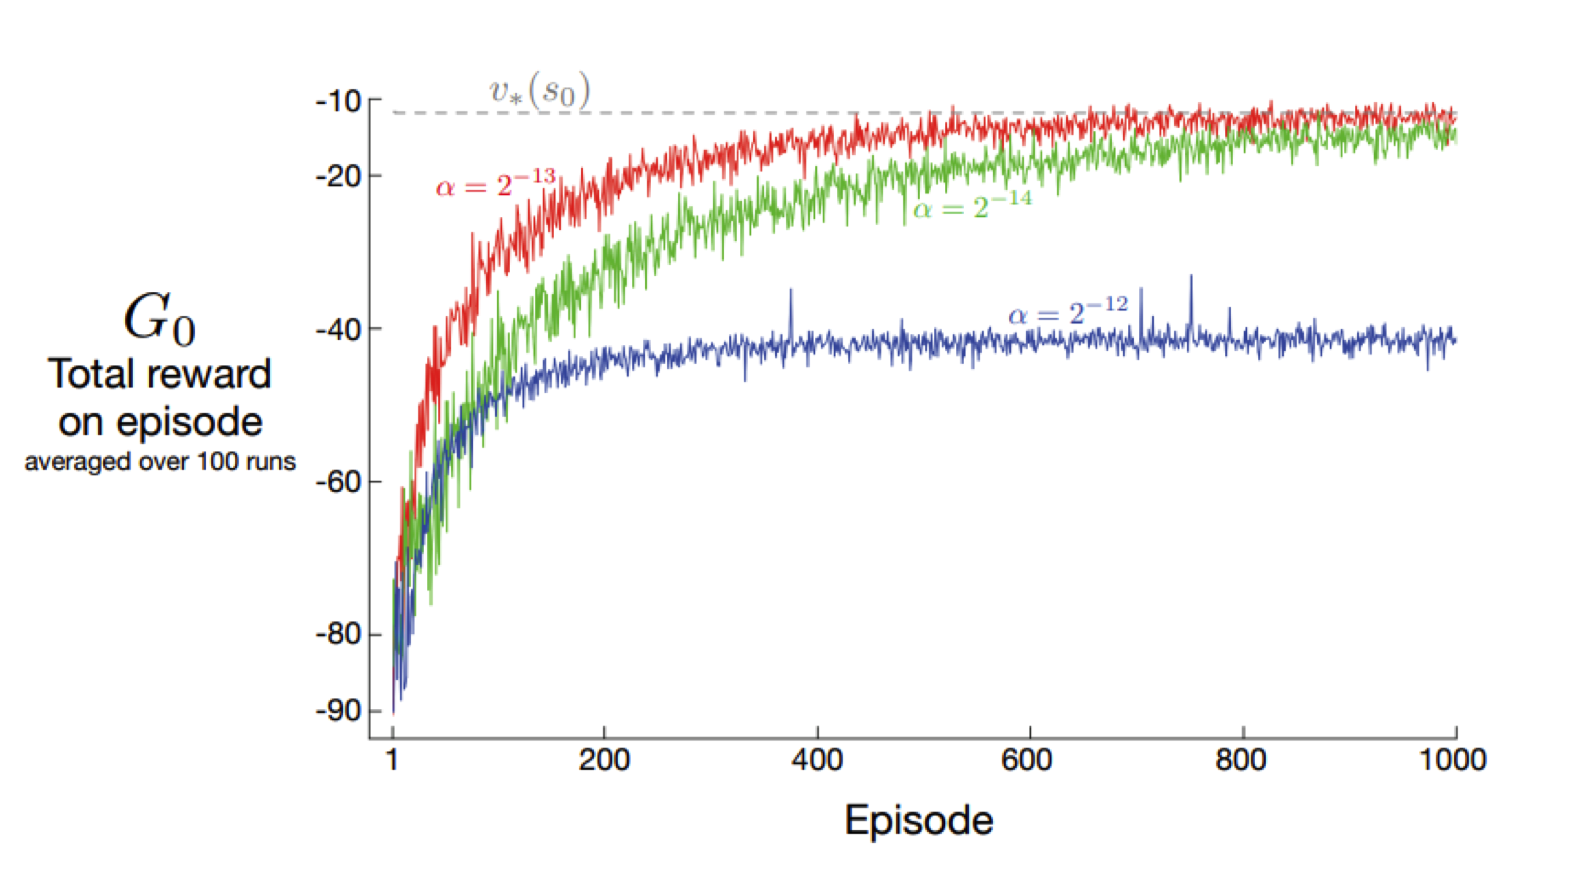
\includegraphics[width=0.8\textwidth]{step_size.png}
    \caption{Step size on convergence time, figure credit to \cite{sutton2018reinforcement}. As seen, an appropriate step size help gradient ascent converge at a good maximum. Too large or too small step size both lead to non-optimal result.}
    \label{fig:my_label}
\end{figure}

\begin{figure}[H]
    \centering
    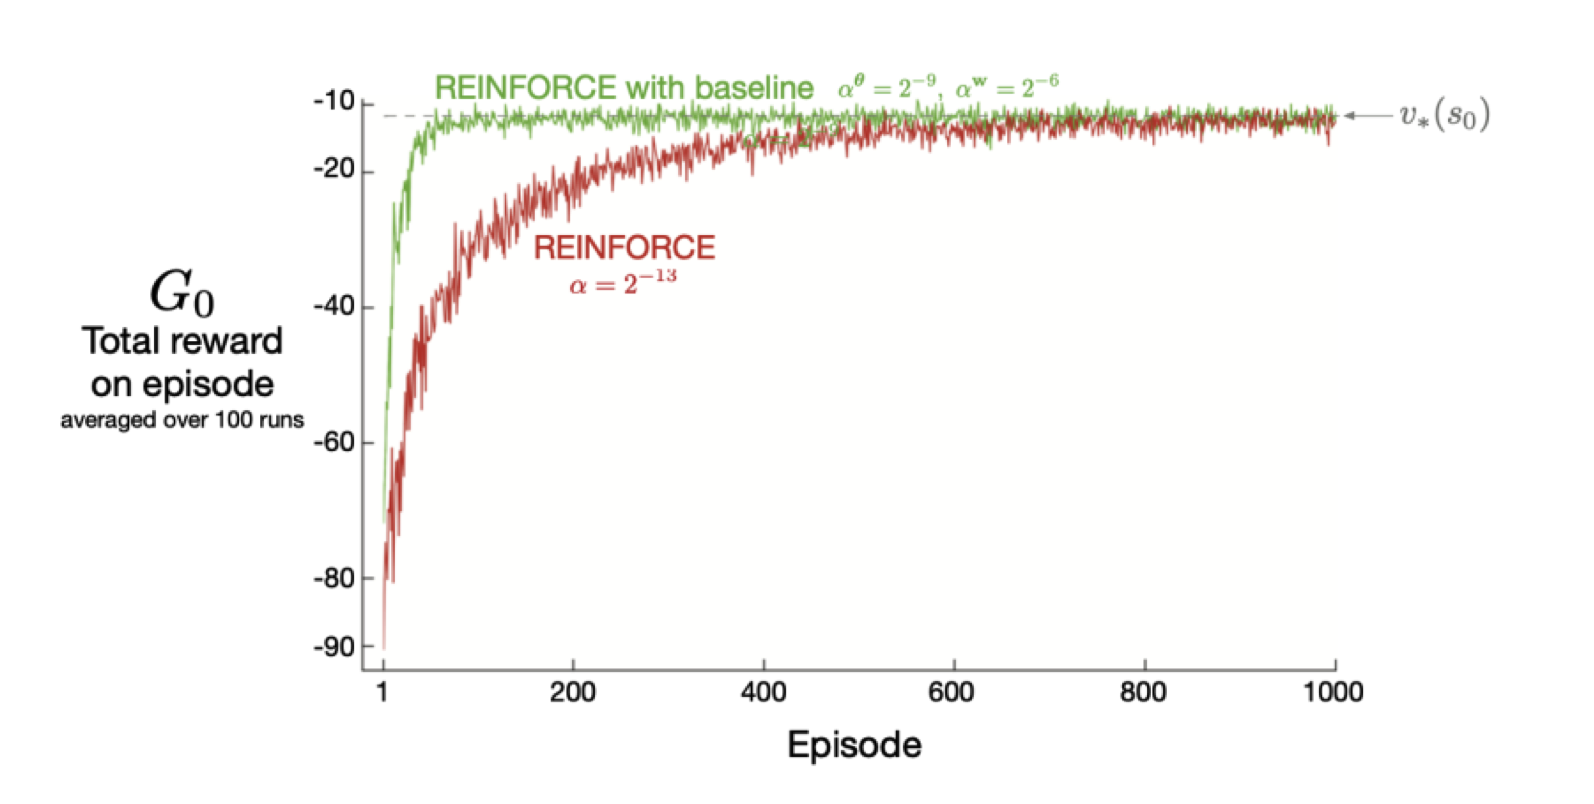
\includegraphics[width=0.8\textwidth]{baseline.png}
    \caption{Baseline offset on convergence time, figure credit to \cite{sutton2018reinforcement}. With the baseline offset trick, the gradient ascent converges much faster.}
    \label{fig:my_label}
\end{figure}

\end{document} % Done!


